\section{Registration and the first use-proof gate}\label{sec:life}

This section uses the largest sample the record allows: every class-record
filed 1995--2018 for the registration step, and every unique registration
issued 2002--2018 for the first use-proof gate. It relates atypicality and
lead to each step, reports how the two steps differ for self-filed and
professionally filed applications, describes how applicants amend a
description between attempts, and closes with the reason the sections that
follow are confined to marks that reached the first gate.

A US trademark passes through a sequence of dated, high-stakes steps, and
each step leaves a record. An application is filed with a goods/services
description; an examiner reviews it, often issuing office actions the
applicant must answer; if allowed and (for intent-to-use filings) a
statement of use is filed, the mark registers. Registration starts a
maintenance clock: in years five to six the owner must file a Section~8
declaration proving continued use in commerce, with a six-month grace
period; around year ten a combined Section~8 declaration and Section~9
renewal is due, and every ten years thereafter. A mark that misses a
use-proof gate is cancelled. Madrid Protocol registrations
(\S66(a) basis) file Section~71 declarations on the same schedule and
are flagged separately throughout. \citet{Graham2013} describe the
administrative data; the event-dated corpus built here adds the full
prosecution history of each case, so a cancellation is assigned to a
specific gate by its date rather than inferred from a status snapshot.

\begin{table}[h]\centering\small
\caption{The trademark funnel in this corpus. Registration counts are
unique serials; gate outcomes are event-dated (a Section~8 cancellation
at registration age 4.0--8.5 years). Source: the re-parsed USPTO
application backfile, scored as in Section~\ref{sec:construct}.}
\label{tab:funnel}
\begin{tabular}{lrr}
\toprule
Stage & $n$ & Share \\
\midrule
Debut filings scored, 1995--2018 (owners' first filings) & 3{,}589{,}068 & \\
\quad reached registration & 2{,}066{,}600 & 57.6\% \\
\midrule
All unregistered class-records filed 1995--2018 & 3{,}798{,}318 & \\
\quad never filed statement of use & & 42.6\% \\
\quad stopped responding in prosecution & & 45.3\% \\
\quad removed adversarially & & 4.3\% \\
\midrule
Registrations 2002--2018, scored, unique serials & 3{,}104{,}534 & \\
\quad failed the first use-proof gate (event-dated) & & 52.3\% \\
\midrule
Passed first gate, cohorts 2002--2013, terminal status known & 1{,}129{,}724 & \\
\quad failed at the year-ten renewal & & 39.1\% \\
\bottomrule
\end{tabular}
\end{table}

The paper relates two properties of a filing's description --- how unusual
its language is for its industry, its \emph{atypicality}, and whether that
language is ahead of or behind where the industry's language was moving, its
\emph{lead} --- to what happened to the filing afterwards. Section~\ref{sec:construct}
builds the two properties. The outcomes are three steps in the sequence above,
each read from the dated record and each bounded as follows.

\emph{Registration.} Whether an application reaches registration at all,
among filings made 1995--2018. Of the applications that do not register,
roughly nine in ten die by the applicant's own inaction --- never filing the statement of use, or going
silent during prosecution --- and only 4.3\% are removed adversarially
(Table~\ref{tab:funnel}), so registration is read as a launch indicator rather
than an examiner's verdict.

\emph{Survival of the first use-proof gate.} Whether a registration was
cancelled for non-use at registration age 4.0 to 8.5 years, among
registrations issued 2002--2018. This is where the market's verdict reaches
the record: half of registered marks do not survive it, and failing it means
the product the mark named is no longer in commerce. Every gate estimate is
conditional on the mark having been granted, because registration is itself
selected on language; what the unconditional composite looks like is shown
once, in Appendix~\ref{sec:robust_uncond}, and not otherwise used.

\emph{Reaching SEC reporting.} Whether the owner of a first-time filing ever
appears in SEC financial-statement records, a firm-level outcome used in
Section~\ref{sec:bluesea} to ask whether either property of the text marks
firms bound for public markets.

Outcomes are rates, so every estimate is a shift in a probability and is
stated in percentage points against the base rate it shifts: $+1.4$pp on a
52.3\% base means 53.7\% against 52.3\%, not 52.3\% multiplied by $1.014$.
The basic comparison is the outcome rate of the fifth of filings with the
highest lead minus that of the fifth with the lowest, with the fifths cut
inside a single industry and year so that no difference between industries or
between years enters; the regression tables add drafting and filer controls
and cluster errors on the owner. Where a continuous version is given, it is
the change in the outcome for a one-standard-deviation change in lead, in
percentage points.

Counting differs by table. A filing may claim several Nice classes at once, so
a \emph{class-record} counts it once per class while a \emph{registration}
counts it once by serial number; a \emph{debut filing} is an owner's first, one
per owner. The funnel above counts debut filings, the gate regressions unique
registrations, the per-class figures class-records.

Three windows bound the samples, each set by an institutional fact. Scoring
runs 1995--2019, because a full
five-year past reference does not exist before 1990 and a full forward
reference does not exist after 2020; the analysis cut of 1995 is about two
years more conservative than the measured burn-in requires
(Appendix~\ref{app:comp}). The gate cohorts end in 2018 because the
cancellation record runs to April 2026 and the failure window closes at
registration age 8.5 years, so 2018 is the last cohort whose window has
essentially elapsed --- the top of that range is fractionally censored, and
a separate 2019 replication is reported below. They begin in 2002 because
that is the conventional cut for this corpus, and that lower
bound turns out to matter: carried back to the first scoreable cohorts the
penalty is two to three times larger than it has ever been since, and
Section~\ref{sec:eras} reports what the restricted window concealed.

Outcomes are read from the event-dated prosecution history, which attributes
each cancellation to a specific gate and observes counsel and basis directly,
and cross-checked against the USPTO status-code dictionary.\footnote{700
registered; 701--705 Section~8 accepted; 710 cancelled for Section~8 failure;
800 renewed; 900 expired.}

\subsection{Registration rewards a middling atypicality}\label{sec:registration}

Across 3.59 million debut filings (57.6\% base rate), completion is an
inverse-U in \emph{atypicality}: it climbs from 46.6\% at the least atypical
end to about 58\% in the middle and falls back to 53.4\% at the most atypical
(Figure~\ref{fig:profiles}, panel C). The same shape appears on the
past-facing level alone, more mildly, running 54.0\% at the bottom quintile to
58.4--59.1\% in the middle and 57.7\% at the top (Figure~\ref{fig:outcomes}A).

The signed axis behaves differently. Completion on \dkl{} falls to a trough of
51.9\% just above the median and then rises steadily to 58.0\% at the leading
end. That trough is composition rather than timing: $|L|$ correlates with
atypicality at $+0.31$, so filings near zero lead are disproportionately
low-atypicality filings, which complete poorly for the reason above. Split by
atypicality, the trough is absent in the upper three fifths and survives in
the lowest. Reference windows built by calendar year put an inverse-U on this
axis too, but that one is an artifact of annual bucketing
(Appendix~\ref{app:rolling}) and does not survive at daily resolution. The
signed axis still enters a linear specification strongly
(Table~\ref{tab:staged}), but monotonically rather than through an interior
peak: what curvature exists at registration belongs to how far a filing's
language sits from its category, not to which side of it the filing sat.

The obvious objection is that unfamiliar language is simply refused more
often, so the measure recovers nothing beyond familiarity. Completion falls at
\emph{both} ends, so the most category-typical filings also complete less than
the middle, which familiarity cannot explain; and the curvature is specific to
the unsigned axis, the signed axis showing no interior peak at all.


\begin{figure}[h]\centering
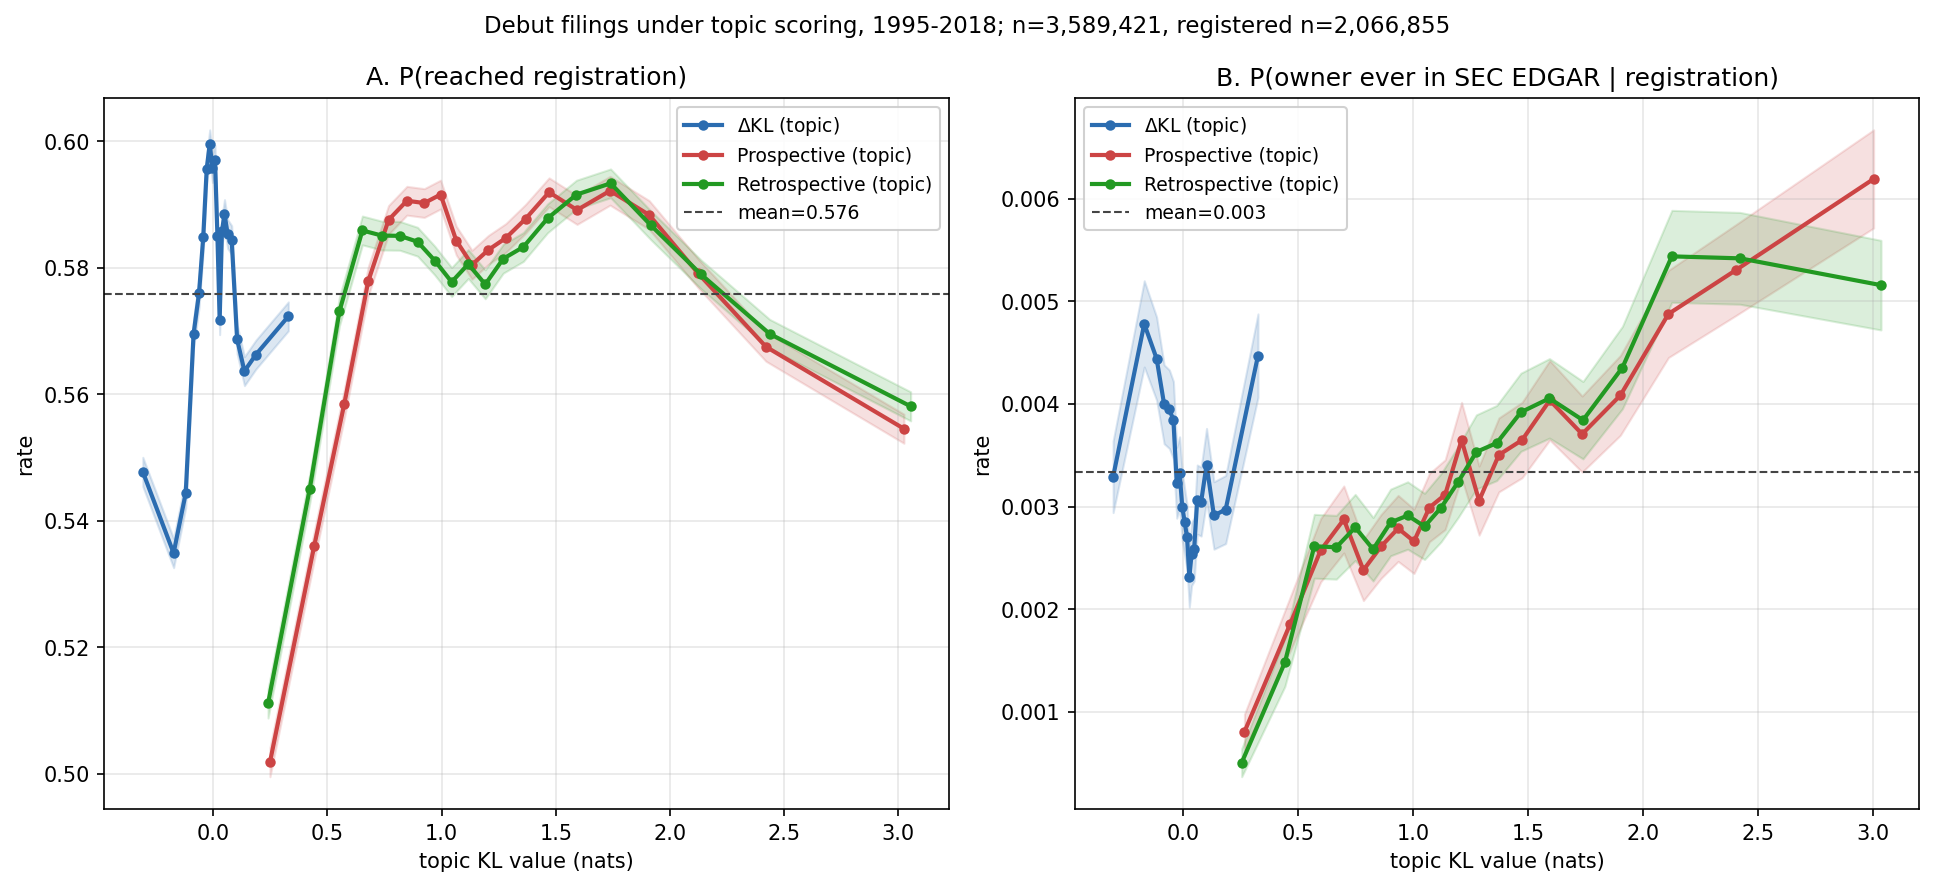
\includegraphics[width=\textwidth]{results/debut_outcome_topic.png}
\caption{Outcomes for debut filings (owner's first-ever filing) across all
45 Nice classes under topic scoring, filing years 1995--2018, in quantile
bins with 95\% intervals. $n = 3{,}589{,}068$; registered subset
$n = 2{,}066{,}600$. \emph{A:} P(reached registration). \emph{B:} P(owner
ever in SEC EDGAR, the Commission's public filing system $\mid$
registration); the structure in panel B is
decomposed in Section~\ref{sec:bluesea}.}
\label{fig:outcomes}
\end{figure}

\begin{figure}[h]\centering
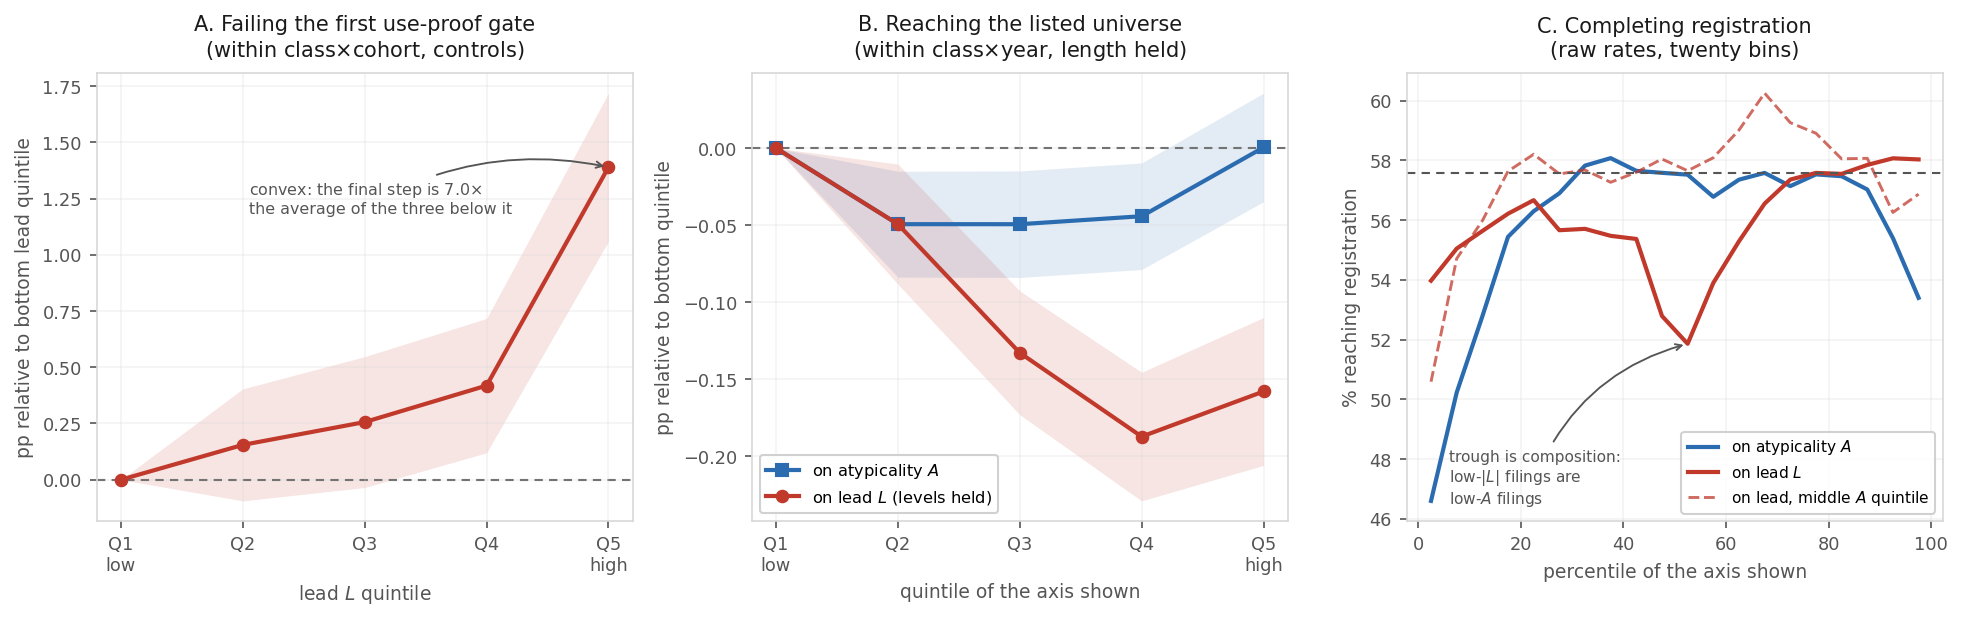
\includegraphics[width=\textwidth]{results/quintile_profiles.png}
\caption{Quintile profiles for the three outcomes. \emph{A:} the share of
registrations failing the first use-proof gate, by lead quintile, adjusted
within Nice class and registration year with the drafting and filer controls
of Table~\ref{tab:gate_lpm}; the dashed line is the rate for all
registrations. The profile rises gently and monotonically through the fourth
quintile and then steps up: about seven tenths of the top-to-bottom gap is
the single step from the fourth quintile to the fifth, seven times the
average step below it. A gradient is present, but the step at the top
dominates it, and the text reports top-versus-bottom contrasts for that
reason. \emph{B:}
the share of first-time filers whose owner ever reaches SEC reporting, by
quintile of atypicality and of lead, adjusted within Nice class and filing
year with description length held; flat in atypicality, and falling in lead
through the fourth quintile once the levels are controlled. Whiskers in A and
B are 95\% intervals on the difference from the bottom quintile. \emph{C:}
raw registration rates for debut filings in twenty bins --- an inverse-U on
atypicality, and on lead a trough just above the median that is
compositional, absent once atypicality is held in its middle fifth (dashed).
Horizontal line at the pooled rate.}
\label{fig:profiles}
\end{figure}

\subsection{Self-filed and professionally filed applications}\label{sec:representation}

Counsel of record is observed on every filing. Represented applications are
73\% of filings over 1995--2018, falling from 85\% in 1995 to 68\% in 2018 as
online self-filing spread. The two populations differ at both steps.
Represented applications reach registration 61.9\% of the time and
self-filed applications 45.6\%. Among registrations, represented marks fail
the first use-proof gate 47.5\% of the time and self-filed marks 69.2\%. The
second gap is the larger, and it is not a drafting effect: the gate is
proof of continued use, so a self-filed registration that fails it names a
product that went out of commerce within six years, and self-filers are
disproportionately new and small.

Self-filers also write differently. Their descriptions are shorter (a median
of 21 terms against 28 in the software class, 17 against 26 in advertising
and retail), sit closer to their class's usual language, and lean slightly
further ahead of it. Representation therefore moves both sides of every
comparison below at once, which is why it is held in every regression and
why the estimates are reported separately by stratum
(Table~\ref{tab:gate_lpm}). Held, the lead penalty is of the same order in
both populations: $+1.8$pp among self-filed registrations and $+1.2$pp among
represented ones.

\subsection{How applications are amended}\label{sec:amend}

An application that is abandoned is usually the end of that attempt: among
2.28 million abandoned applications, 3.6\% are followed within six years by
the same owner filing the same mark again in the same class, and 1.5\% by
one that then registers. The refilings that do occur show what an applicant
changes. Of the 42{,}115 abandoned applications whose owner later registered
the same mark in the same class, 74\% carry a different goods/services
description the second time. Scoring each registration on the text it was
first tried with and on the text it registered with gives the direction of
the change. Both self-filers and represented owners rewrite toward the
class's typical description: originals in the most atypical fifth lose
$0.39$ nats of atypicality, and originals in the most conventional fifth
gain $0.16$. Refilings that reuse the identical text move by less than
$0.01$ at every position, so the convergence is in the writing.
Representation changes the extent but not the direction: owners who hire
counsel for the second attempt rewrite most often (82\%) and their
descriptions lengthen by 16\%; counsel rewriting their own earlier draft
rewrite least often (72\%) and shorten by 4\% (Appendix~\ref{app:refile}).
Lead barely moves once the windows' shift with the later date is taken out.

Applicants therefore adjust descriptions to resemble what the class already
files. A registered description is in part a conformed one, and the
atypicality of registered marks is compressed relative to what applicants
first wrote. Every estimate on registered marks is an estimate on conformed
language. The refiled cases themselves move nothing: they are $1.1$\% of the
gate sample, they fail it slightly less often than other registrations
(51.7\% against 52.8\%), and the within-class-and-year contrast is $+2.25$pp
with them and without them.

\subsection{Leading marks fail the first use-proof gate}\label{sec:gate}

Marks written in language their industry subsequently moved toward fail
their first use-proof gate more often than marks written in language it was
moving away from. Within Nice class and registration year, controlling for whether the
filer drafted the mark themselves or hired counsel, and for the length of the
description, marks whose language most leads their industry fail $1.4$
points more often (53.3\%) than those in the most lagging fifth (51.9\%;
$t = 8.3$, Table~\ref{tab:gate_lpm}).

Among 4.12 million registration class-records 2002--2018, dated first-gate cancellation rises from 50.0\%
at the bottom topic-\dkl{} quintile to 52.4\% at the top, positive in 33
of 44 classes with sufficient volume (Figure~\ref{fig:forest}). But a raw
pooled contrast mixes the within-industry gradient with class and registration-year
composition, treats multi-class registrations as independent observations,
and ignores that gate outcomes correlate within owner. The
primary estimates therefore come from a linear probability model on 3.10
million unique registrations, one row per serial, with \dkl{} quintiles cut
\emph{within} Nice class and registration year. The specification adds
class$\times$registration-year fixed effects; controls for counsel of record,
intent-to-use basis, log description length, log owner filing volume, owner
domicile, and foreign filing basis;\footnote{A US application is filed
either on \emph{use} --- the mark is already in commerce --- or on
\emph{intent to use}, which defers proof until after allowance. Foreign
applicants may instead file on a home registration (\S44(e)) or extend an
international registration into the US under the Madrid Protocol
(\S66(a)); the latter maintain under \S71 rather than \S8. These are
statutory routes to the same registration, and they differ sharply in who
files and how often the mark is abandoned, which is why each enters as a
control.} and standard errors clustered on 1.27
million normalized owners (Table~\ref{tab:gate_lpm}).\footnote{Ties are
common. Within the class$\times$registration-year cell the quintiles are cut in,
$17.1$\% of scored registrations share a \dkl{} value with at least one
other filing, and the largest tie group runs to 53. Anchoring the reference
window on the filing date does not remove them, because filings that share a
class, a filing date and a goods/services description --- an owner
registering a family of marks at once, on Manual language --- have identical
distributions scored against identical references. Cut points are fixed by
sorting on the score and then on the serial number, which is reproducible
but systematic: serials run in filing order. It makes no difference. Sorting
the ties the opposite way moves the top-versus-bottom contrast by $0.001$pp,
and five pseudorandom orderings move it by at most $0.002$pp, against a
contrast of $2.287$pp --- a tenth of one percent of the estimate.}

\begin{table}[h]\centering\small
\caption{First-gate failure and \dkl{}: design-based estimates.
LPM of event-dated first-gate failure on within-class$\times$registration-year
\dkl{} quintiles (Q1 omitted), unique serials, registrations 2002--2018.
Failure is a dated cancellation for non-use at registration age 4.0--8.5
years, under \S8 or, for Madrid \S66(a) registrations, \S71.
All specifications include class$\times$registration-year fixed effects; controls
are counsel of record, intent-to-use basis, log goods/services length,
log owner filing count, owner domicile (US, CN), and foreign basis
(\S44(e), \S66(a)). Base failure rate 52.3\% on this sample.}
\label{tab:gate_lpm}
\begin{tabular}{llrrr}
\toprule
Sample & Specification & Q5$-$Q1 (pp) & SE & $n$ \\
\midrule
All & FE only & $+2.29$ & $0.16$ & 3{,}104{,}534 \\
All & FE + controls & $+1.39$ & $0.17$ & 3{,}104{,}534 \\
Counsel-represented & FE + controls & $+1.15$ & $0.20$ & 2{,}414{,}318 \\
Counsel + US-domiciled & FE + controls & $+1.60$ & $0.22$ & 1{,}888{,}352 \\
Self-filed & FE + controls & $+1.80$ & $0.26$ & 690{,}216 \\
Excluding Madrid \S66(a) & FE + controls & $+1.82$ & $0.18$ & 2{,}924{,}427 \\
\midrule
Counsel + US, 2002--07 & FE + controls & $-0.25$ & $0.33$ & 551{,}989 \\
Counsel + US, 2008--12 & FE + controls & $+2.00$ & $0.42$ & 551{,}924 \\
Counsel + US, 2013--18 & FE + controls & $+2.65$ & $0.25$ & 784{,}439 \\
\midrule
All & continuous, pp per sd of lead & $+0.58$ & $0.05$ & 3{,}104{,}534 \\
Counsel + US & continuous, pp per sd of lead & $+0.63$ & $0.06$ & 1{,}888{,}352 \\
\bottomrule
\end{tabular}
\\[0.3em]\footnotesize Standard errors replace significance stars: with $n$
in the millions every coefficient has $p < 0.01$, so stars would mark each
row identically. Errors are clustered on \emph{normalized owner} --- names
uppercased, stripped of punctuation and of twenty legal suffixes, so
\textsc{acme corp.} and \textsc{acme corporation} are one cluster. A single
owner files many marks, drafts them in a house style, and abandons them
together when the business fails; the within-owner correlation of gate
survival is $0.42$, so the 1.27 million owner clusters, not the filings,
carry the information. The Madrid row drops \S66(a) registrations rather
than absorbing them in a control, since they maintain under a different
statute; the estimate is larger without them.
\end{table}

The gradient is monotone within cells. Whether the filing was drafted by
counsel or by the owner is held because it moves both sides of the
comparison at once: self-filers fail the gate at 69.6\% against 46.8\% for
represented owners, and they write shorter descriptions that sit closer to
their class's usual language yet lean slightly further ahead of it, so
without the control, part of any lead gradient is a self-filing gradient. With it, the penalty is of the same order in both
strata ($+1.8$pp self-filed, $+1.2$pp counselled). The full control set cuts the
magnitude by about a third without absorbing it, and the estimate is if
anything \emph{largest} in the cleanest stratum --- counsel-represented,
US-domiciled owners --- so it is not carried by the self-filed or foreign
mass-filing segments whose gate failure rates are high for their own
reasons.\footnote{The level effects on those covariates are large in their
own right: counsel $-19.5$pp and Madrid \S66(a) basis $+10.3$pp.} About
forty percent of the raw pooled contrast is composition: $+1.4$pp
design-based against $+2.5$pp raw.

\begin{figure}[h]\centering
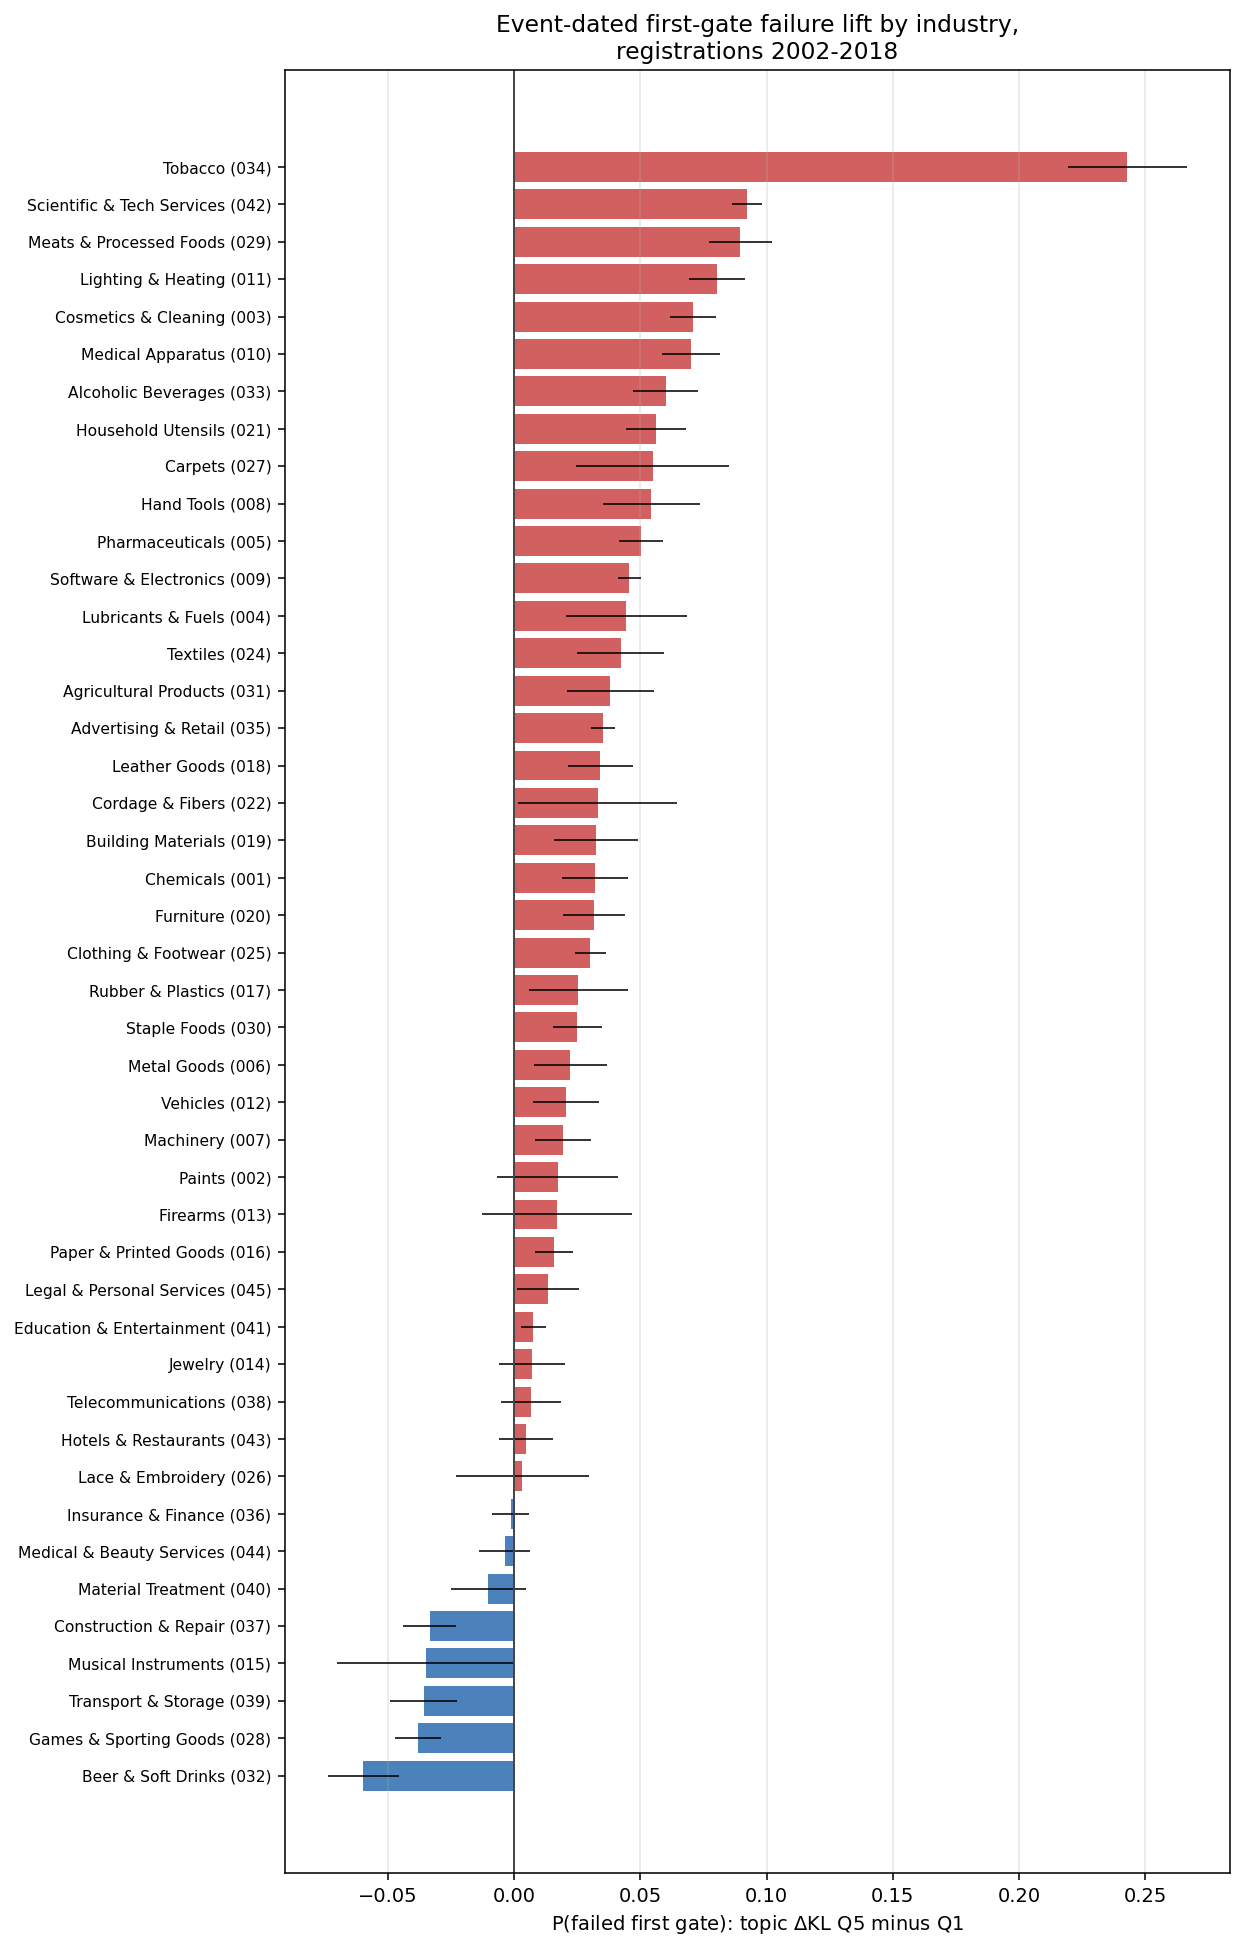
\includegraphics[width=0.72\textwidth]{results/event_gate_forest.png}
\caption{Event-dated first-gate failure lift (topic \dkl{} top minus
bottom quintile) by industry, registrations 2002--2018, raw quintile
contrasts. Positive bars indicate the leading penalty. Whiskers are
two-sample binomial intervals, uncorrected for the within-owner correlation
($0.42$) and so narrower than clustered intervals; read
Table~\ref{tab:gate_lpm} for precision. Per-class breakouts are in the
online appendix.}
\label{fig:forest}
\end{figure}

Within the 2002--2018 window the penalty looks modern: indistinguishable
from zero for the 2002--2005 cohorts, turning positive in 2006, and running
$+1.8$ to $+5.6$pp for every cohort from 2008 onward
(Figure~\ref{fig:cohort}). That reading does not survive carrying the
series back: the penalty was two to three times larger for the earliest
scoreable cohorts than for any since, which makes the 2002--2005 quiet a trough
between two episodes rather than a starting point (Section~\ref{sec:eras}).

The gate is close to a fixed appointment rather than a hazard spread over years: of the 1.35 million
cancellations recorded for fully observed cohorts, 17 post before
registration age 6.5, 96.1\% post between 6.5 and 7.0, and the rest after
seven. Since the cancellation record ends on 2 April 2026, a cohort is
observable only once it has reached seven years, which makes 2019 the last
one with usable gate data and leaves 2020 and later with no observed gate at
all. Measured on the 6.5--7.0 band, fully observed for every cohort it
covers, the penalty runs between $+2.1$ and $+5.6$pp with no trend across
the decade and overlapping intervals at its two highest points. The 2019
reading rests on the 78{,}408 registrations issued early enough in that year
to reach seven years inside the record, so it is a first-quarter subsample
rather than a cohort.

The outcome is an indicator on a window, so a mark that fails outside it
counts as a survivor. If leading marks failed at the same rate as lagging ones
but sooner, that alone would put them inside the window more often and the
measure would report a difference in rates where there was only a difference in
timing. It is not.
On the 3.15 million registrations whose ninth anniversary is inside the
record --- for which failure is settled and no window is needed --- the
contrast is $+2.71$pp within class and registration year, against $+2.65$pp on the
paper's 4.0--8.5 window and $+2.65$pp on the narrow band. Conditional on failing, the probability of failing late
carries a contrast of $-0.01$pp ($t = -0.2$) once class and registration year are
held. The pooled version of that contrast is $+0.27$pp and is composition.

The filer population changed over the same period. Within
counsel-represented US-domiciled owners, and with the full control set, the
earliest cohort third is slightly negative ($-0.25$pp, SE $0.33$) while the
two later thirds are clearly positive ($+2.00$ and $+2.65$pp,
Table~\ref{tab:gate_lpm}). The gradient is therefore not an artefact of the
post-2015 surge in self-filed and foreign applications.

\begin{figure}[h]\centering
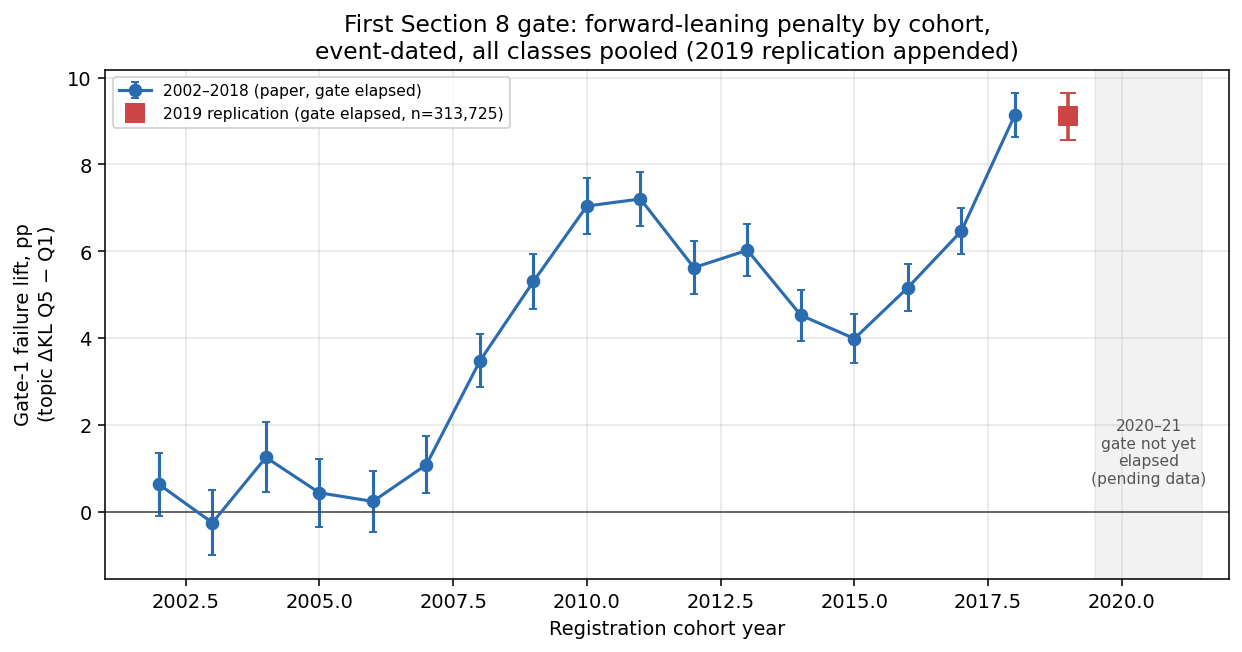
\includegraphics[width=0.8\textwidth]{results/event_gate_cohort_curve_extended.png}
\caption{The leading gate penalty by registration cohort, all classes
pooled. Each point is the event-dated first-gate failure rate of the most
leading fifth of that cohort's registrations minus that of the most lagging
fifth, with lead quintiles cut within the cohort and no controls. The penalty is
absent or negative for the 2002--2005 cohorts, turns positive in 2006, and
is present in every cohort from 2008 through 2019, ranging $+1.8$ to
$+5.6$pp with no downward trend. 2019 is the last evaluable cohort:
cancellations post at about age six and a half and the record ends in April
2026, so later cohorts have not reached their gate rather than having
passed it.}
\label{fig:cohort}
\end{figure}

\subsection{The penalty is not modern, and it is not general}\label{sec:eras}

Scores exist from 1995 on, which makes registration cohorts from 1996 evaluable, and their gate
outcomes have been settled for two decades. Carried back, the contrast runs
$+6.9$pp for the 1996 cohort and rises to $+10.1$pp for 1999 --- two to
three times anything observed since --- then collapses. The 2002--2005
cohorts the paper had been reading as a quiet baseline are a trough between
two episodes, and one of them is the larger.

Scores begin in 1995, so a 1996-cohort registration must have issued within
a year of filing; early cohorts are selected on prosecution speed, and speed
plausibly travels with drafting in standard language. Holding pendency in a
common one-to-three-year band leaves the series unchanged. Indexing by
filing year instead, so a cohort contains every prosecution speed, gives
$+7.9$ to $+9.6$pp for filings 1995--1999 and $-0.95$pp for filings made in
2000 --- a ten-point swing in a single filing year.

Splitting the four classes that carry most technology filings --- 009, 035, 038 and 042 ---
against the other forty-one separates a large moving component from a small
steady one (Figure~\ref{fig:eras}):

\begin{center}\small
\begin{tabular}{lrr}
\toprule
Filing years & Technology classes & All others \\
\midrule
1995--1999 & $+14.18$ (0.36) & $+4.48$ (0.27) \\
2000--2004 & $-1.37$ (0.35) & $+1.21$ (0.24) \\
2005--2007 & $+2.04$ (0.43) & $+1.99$ (0.28) \\
2008--2014 & $+9.02$ (0.25) & $+1.32$ (0.17) \\
\bottomrule
\end{tabular}
\end{center}

\noindent Outside technology the penalty is a flat $+1$ to $+4$pp in every
era, including the one in which the pooled series reads as zero. Inside
technology it swings by fifteen points: strongly positive for filings made
into the late 1990s, negative for those made in the five years after, and
positive again from 2008. The pooled null of 2002--2005 is a technology
reversal partly offsetting a non-technology positive, not an absence.

What this design cannot say is which cycle the swing belongs to. Marks filed
1995--1999 reach their gate in 2001--2007 and marks filed 2000--2004 reach
theirs in 2006--2013, so a story in which unusual language is punished
because it was written during an investment boom and a story in which it is
punished because the gate falls during a bust both fit these numbers.

\begin{figure}[h]\centering
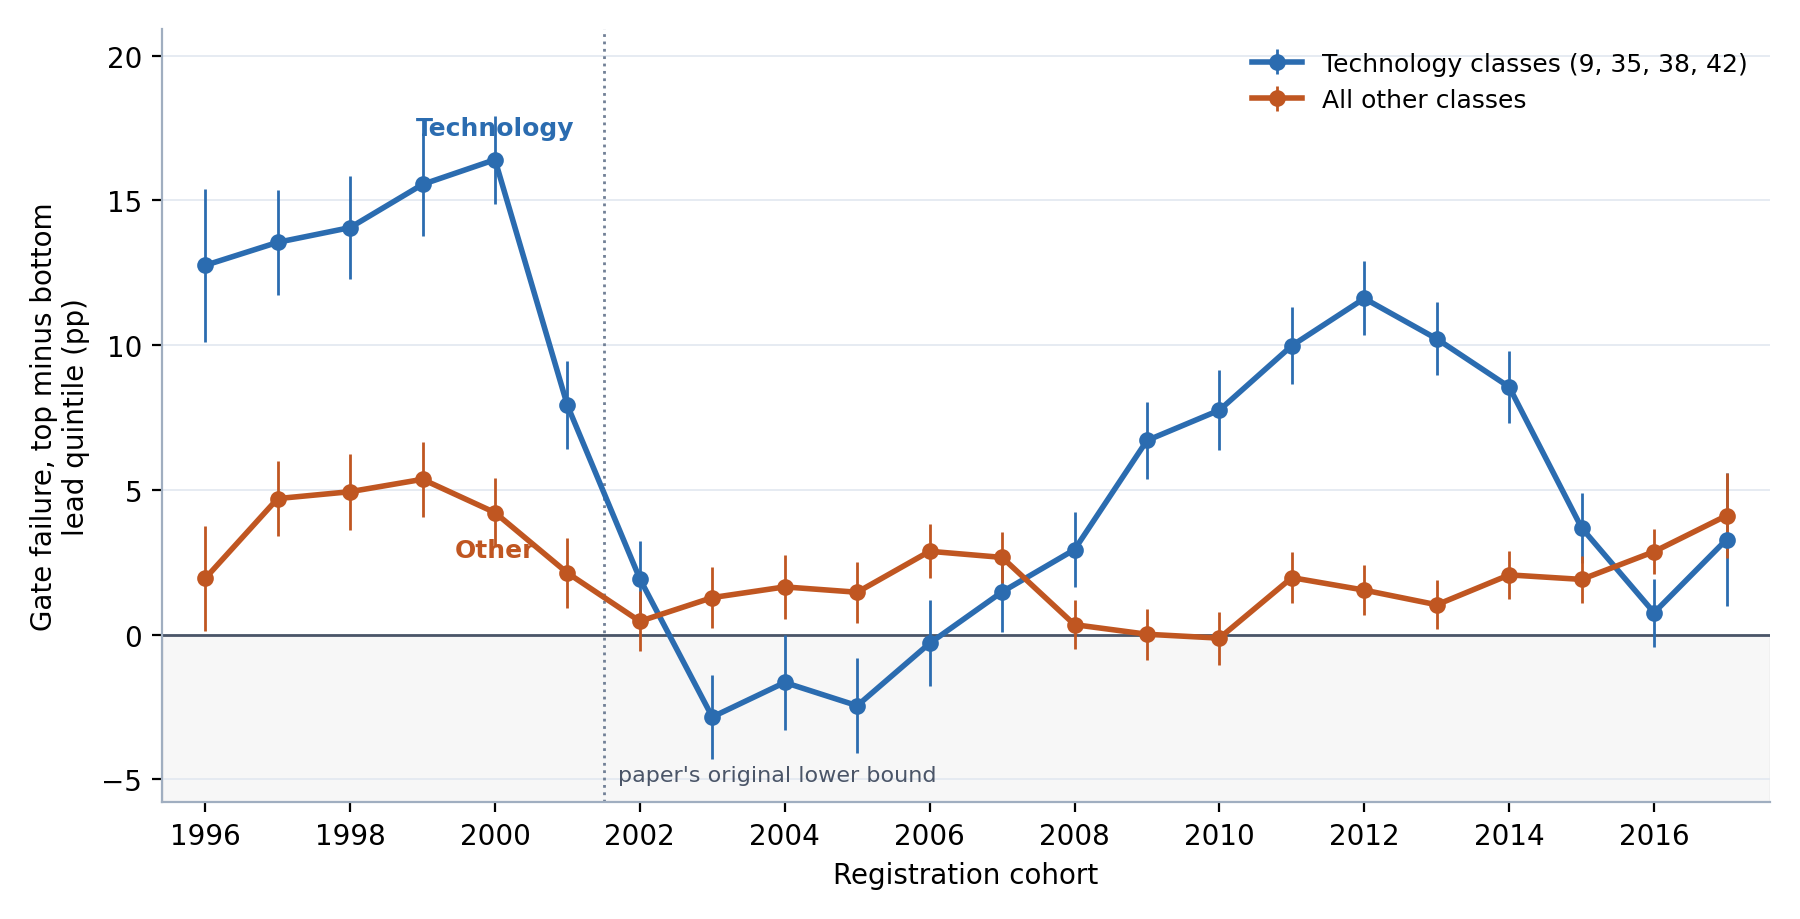
\includegraphics[width=0.86\textwidth]{results/gate_era_profile.png}
\caption{The leading gate penalty by registration cohort, technology classes
(009, 035, 038, 042) against all others. Each point is the first-gate failure
rate of the most leading fifth of that cohort's registrations minus that of the
most lagging fifth, lead quintiles cut within cohort and group, no controls,
with 95\% intervals. Cohorts are
restricted to registrations whose ninth anniversary is inside the record, so
every outcome shown is settled. Outside technology the penalty is small and
almost flat across two decades; inside technology it swings from $+16$pp for
the 2000 cohort to $-3$pp for 2003 and back to $+12$pp for 2012. The dotted
line marks the 2002 cut that the main cohort series uses.}
\label{fig:eras}
\end{figure}

\subsection{Three of the four classes reverse, and the leading language changes theme}\label{sec:techswing}

The four-class split pools industries that do not move together. Taking
them one at a time, and then assigning quintiles inside progressively finer
cells (Table~\ref{tab:techswing}):

\begin{table}[h]\centering\small
\caption{The leading gate penalty inside technology, by class and by cell.
Top-minus-bottom lead-quintile contrast in first-gate failure (pp, SE in
parentheses), settled registrations, by filing era. The upper block assigns
quintiles within each class and era. The lower block pools the four classes
and assigns quintiles within the era (raw, as in the text table above),
within class$\times$registration-cohort cells, and within
theme$\times$class$\times$registration-year cells, where a filing's theme is the one
its description loads most heavily on under the production $T = 50$ model.
$n = 1{,}248{,}591$.}
\label{tab:techswing}
\begin{tabular}{lrrrr}
\toprule
Class & 1995-1999 & 2000-2004 & 2005-2007 & 2008-2014 \\
\midrule
009 Electrical, software & $+18.04$ (0.52) & $-5.32$ (0.51) & $+0.25$ (0.62) & $+11.67$ (0.37) \\
035 Business services & $+4.59$ (0.69) & $-9.70$ (0.56) & $+2.02$ (0.63) & $+1.66$ (0.36) \\
038 Telecommunications & $+9.91$ (1.40) & $-4.24$ (1.29) & $+2.60$ (1.48) & $+3.42$ (0.94) \\
042 Scientific, computer services & $+17.11$ (0.57) & $+6.70$ (0.62) & $+8.42$ (0.87) & $+12.63$ (0.47) \\
\midrule
Four classes pooled, raw & $+14.49$ (0.33) & $-1.81$ (0.31) & $+2.56$ (0.38) & $+9.16$ (0.22) \\
\quad within class$\times$cohort & $+14.27$ (0.33) & $-3.63$ (0.31) & $+2.73$ (0.38) & $+7.24$ (0.22) \\
\quad within theme$\times$class$\times$cohort & $+4.78$ (0.33) & $-1.26$ (0.31) & $+2.56$ (0.38) & $+4.51$ (0.22) \\
\bottomrule
\end{tabular}

\end{table}

\noindent Electrical and software goods (009) and telecommunications (038)
follow the pooled pattern. Business services (035), the class that holds
online retail, reverses hardest: $-9.7$pp for filings made 2000--2004 against
$+4.6$pp in the five years before. Scientific and computer services (042)
never reverses. Its contrast is $+6.7$pp in the era in which the other three
are negative and between $+8$ and $+17$pp in every other, and by registration
cohort it never falls below $+3$pp (Figure~\ref{fig:techswing}). The
reversal is an event in goods and in business services; the class that
sells technology as a service sat it out.

Assigning quintiles within class and registration year rather than within the era
pool changes little. Assigning them within theme, class and registration year
changes a great deal: the late-1990s contrast falls from $+14.5$ to
$+4.8$pp, the post-2008 contrast from $+9.2$ to $+4.5$pp, and the 2000--2004
reversal from $-3.6$ to $-1.3$pp. Two thirds of the first and half of the
second are between themes rather than within them. The leading fifth of each
era was drawn from particular themes, and those themes carried their own
failure rates; the penalty for being leading \emph{inside} a theme is a
steadier $+2.5$ to $+5$pp, the same order as the penalty outside technology.

Which themes is a matter of record (Table~\ref{tab:techthemes}). In
1995--1999 the computer, software, information and data services theme held
38\% of technology filings and 75\% of the leading fifth, and its
registrations failed at 58.9\% against 46--53\% in the other large themes.
That one theme is most of the late-1990s penalty. In 2000--2004 it held
12\% of the leading fifth. The leading language had moved to video, music
and games on electronic media (31\% of the leading fifth against 12\% of
filings) and the internet-services language had become lagging --- wording
the class was leaving --- and inside several themes the lagging fifth now
failed more than the leading one: $-3.6$pp in electronic media, $-5.5$ in
retail store services, $-6.9$ in apparatus and control systems. From 2008
the leading fifth over-represents downloadable and online software by four
to one (15\% against 4\%), the vocabulary of the application store; those
registrations fail at 67.2\%, the highest base rate of any theme, and carry
the largest within-theme contrast anywhere in the table, $+8.4$pp. The
computer-services theme's own contrast, meanwhile, is positive in every era
($+3.6$ to $+5.9$pp) and never reverses.

\begin{table}[h]\centering\footnotesize
\caption{The leading gate penalty by theme within the four technology
classes. Themes with at least 20{,}000 settled registrations, labelled by
their five highest-probability terms; quintiles assigned within theme and
era. Cells with fewer than 3{,}000 registrations are blank.}
\label{tab:techthemes}
\begin{tabular}{p{5.2cm}rrrrr}
\toprule
Theme (top words) & $n$ & 1995-1999 & 2000-2004 & 2005-2007 & 2008-2014 \\
\midrule
services, computer, software, information, data & 451,253 & $+3.61$ (0.52) & $+3.56$ (0.49) & $+4.18$ (0.64) & $+5.92$ (0.37) \\
video, computer, electronic, music, games & 162,290 & $+2.53$ (0.97) & $-3.62$ (0.89) & $-2.85$ (1.01) & $+3.36$ (0.60) \\
services, featuring, store, retail, store services & 131,107 & $+8.39$ (1.09) & $-5.49$ (1.01) & $+2.92$ (1.15) & $+0.98$ (0.66) \\
services, field, training, estate, educational & 95,602 & $+7.82$ (1.09) & $+0.99$ (1.12) & $+6.02$ (1.43) & $+2.05$ (0.83) \\
apparatus, systems, devices, electronic, control & 84,121 & $+4.80$ (1.27) & $-6.92$ (1.19) & $-0.58$ (1.41) & $+3.65$ (0.88) \\
design, field, systems, development, services & 32,517 & $+10.40$ (2.03) & $+4.67$ (1.82) & $+1.50$ (2.27) & $-2.27$ (1.45) \\
software, online, downloadable, non-downloadable, virtual & 29,472 & --- & --- & --- & $+3.30$ (1.05) \\
bags, clothing, shirts, jackets, leather & 28,421 & $+1.28$ (2.59) & $-1.55$ (2.39) & $-4.66$ (2.40) & $+6.06$ (1.36) \\
research, medical, scientific, testing, purposes & 25,897 & $+12.65$ (2.66) & $+12.09$ (2.03) & $-3.82$ (2.59) & $+5.63$ (1.51) \\
services, health, field, care, information & 22,880 & $+4.94$ (2.04) & $+1.39$ (2.36) & --- & $+3.50$ (1.72) \\
\midrule
All themes, within theme$\times$class$\times$cohort & 1,150,921 & $+4.78$ (0.33) & $-1.26$ (0.31) & $+2.56$ (0.38) & $+4.51$ (0.22) \\
\bottomrule
\end{tabular}

\end{table}

\begin{figure}[h]\centering
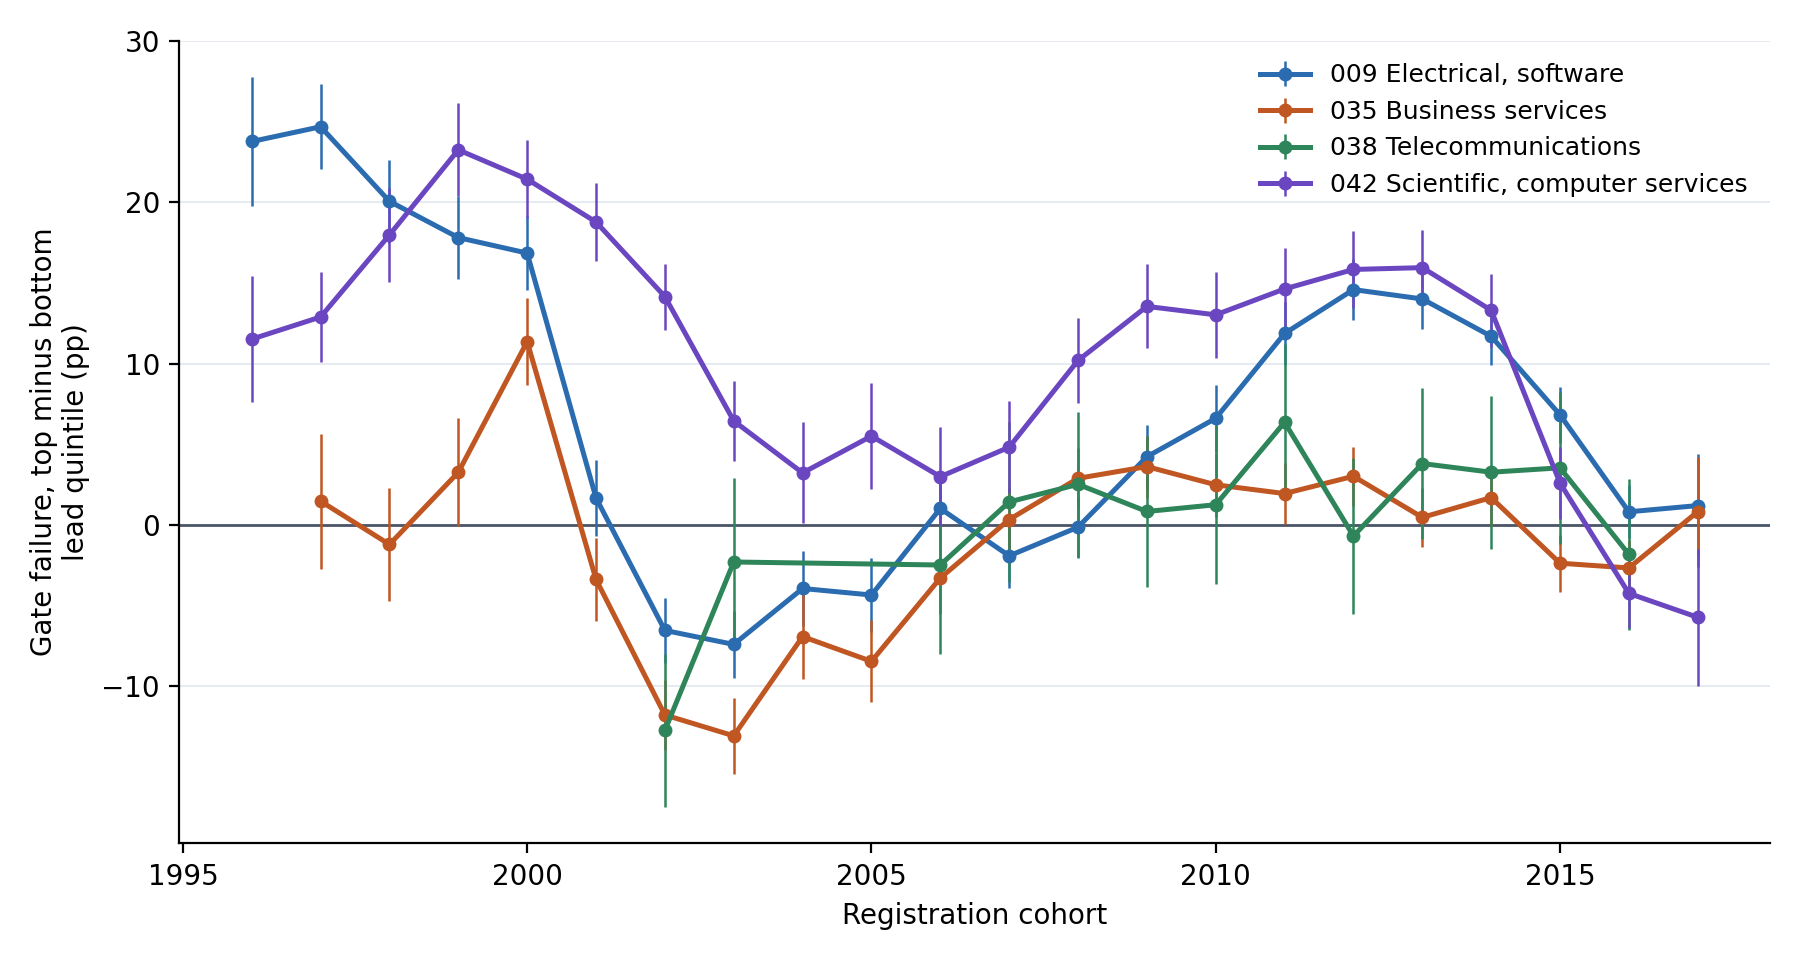
\includegraphics[width=0.92\textwidth]{results/gate_era_tech_themes.png}
\caption{The leading gate penalty by registration cohort, one line per
technology class. Each point is the first-gate failure rate of the most
leading fifth of that class and cohort's registrations minus that of the most
lagging fifth --- lead quintiles cut within class and cohort, no controls ---
with 95\% intervals, on registrations whose gate outcome is settled. Three
classes cross zero between 2001 and 2006; scientific and computer services
does not.}
\label{fig:techswing}
\end{figure}

So the swing has two layers. Across the whole period, a leading filing is a
few points more likely to fail than a lagging one in the same theme, class
and cohort, in technology as elsewhere. On top of that, each era's leading
vocabulary was concentrated in one or two themes whose marks failed at
their own rate: internet services in the 1990s, application software after
2008. In the trough between, the language that had been leading became
lagging, and the marks still written in it failed with it. The
design-based estimates in Table~\ref{tab:gate_lpm} hold class and cohort
fixed but not theme, so they carry both layers; a reader who wants only the
within-theme penalty should take the lower block of Table~\ref{tab:techswing}
as the guide to its size.

Levels and gradients separate cleanly across filer strata. Self-filers
fail the gate far more often than represented owners (69.6\% versus
46.8\%), and intent-to-use registrations more often than use-based ones
(53.1\% versus 50.2\%),
but the \dkl{} gradient itself is similar across these strata once class,
cohort, and drafting covariates are held fixed ($+1.8$pp self versus
$+1.2$pp counseled in Table~\ref{tab:gate_lpm}). Per class, the largest penalties sit in tobacco ($+26$pp, the
vaping era), hand tools ($+10$pp), processed foods ($+10$pp) and medical
apparatus ($+9$pp), with negative lifts in beverages, transport and
construction.

The risk persists at the year-ten renewal, and on the design-based
estimates does not attenuate: the lead coefficient is $-0.49$pp at the first
gate and $-0.63$pp at the second (Table~\ref{tab:staged}). What attenuates is
the raw single-class contrast. In the
software diagnostic class, where the event-dated first-gate lift on the
2010--2013 cohorts reaches $+12.1$pp, the conditional lift at the second
gate falls to $+7.6$pp. Pooled across classes the second-gate profile is not
a slope at all. Fitted over 872{,}079 first-gate survivors with a resolved
year-ten status, a straight line through renewal against lead explains 1\% of
the variation across forty bins and a V explains 89\%
($\Delta$AIC $= 83$, the largest margin anywhere in this paper). Renewal is
highest at both ends of the lead axis and lowest just below its centre. The
$-0.63$pp linear coefficient reported for that row is therefore close to
meaningless as a description, though it is not wrong about the direction of the
leading tail. By year ten the lagging tail has closed the gap in cumulative
failure, having simply taken longer to get there. Most of the difference
resolves at first proof of use.

A competing reading is that the gate measures disengagement rather than
products: an owner who has lost interest both answers the examiner slowly
and lets the registration lapse. The prosecution record tests this through
the gap between the first non-final office action and the response to it.

Response speed does not predict the gate. Across the 1.22 million scored
registrations with a usable office-action/response pair, gate passage varies
between 46.1\% and 48.1\% across response-speed quintiles, from a median of
seven days to 183 --- flat, and if anything the quickest responders pass
slightly \emph{less}. The lead penalty is present in both halves: $-3.48$pp
($\pm 0.40$) among faster-than-median responders and $-2.36$pp ($\pm 0.40$)
among slower, against $-2.94$pp pooled. The restriction drops 61\% of
the sample, disproportionately applications that never drew a refusal, so
this speaks to the prosecuted subset.

Mixing the past and future reference windows identifies which kind of
novelty the gate punishes. Scored against a long past and a short future,
so that lead measures a break with what the class had established, the
top-versus-bottom contrast is $+3.0$pp; scored against a short past and a
long future, so that it measures resemblance to where the class was
heading, it is $+1.65$pp. The symmetric five-year measure sits between, and
the penalty rises monotonically along the mix. The gate punishes breaking
with the past more than it punishes anticipating the future, but it
punishes both (Appendix~\ref{app:comp}).

\subsection{Internet as a theme: web-based filings against their class}\label{sec:internet}

A filing is internet-bearing when its goods/services text names the
internet, the web, a website, online or on-line provision, or electronic
commerce. The rule reads the text rather than the class, so a web retailer
filing in apparel is caught and a semiconductor maker filing in class 009 is
not. Internet-bearing filings are 16.9\% of scored registrations overall:
58\% in telecommunications, 39--41\% in advertising and retail, scientific
and technical services, and legal and personal services, under 5\% in most
goods classes. Table~\ref{tab:internet} gives, for every class, the
registration rate and the first-gate failure rate of internet-bearing
filings against the rest of the class; Figure~\ref{fig:internet} draws the
gate column.

\begin{table}[h]\centering\footnotesize
\caption{Internet-bearing filings against the rest of their Nice class.
Registration is the share of class-records filed 1995--2018 that reached
registration; gate failure is the share of unique registrations 2002--2018
cancelled for non-use at age 4.0--8.5 years. Classes with fewer than 500
internet-bearing registrations are omitted.}
\label{tab:internet}
\begin{tabular}{llrrrrr}
\toprule
Class & & Web share & \multicolumn{2}{c}{Registration (\%)} & \multicolumn{2}{c}{Gate failure (\%)} \\
 & & (\%) & web & rest & web & rest \\
\midrule
001 & Chemicals & 1.8 & 65.0 & 64.3 & 46.1 & 39.1 \\
003 & Cosmetics \& Cleaning & 2.8 & 58.0 & 54.2 & 52.1 & 54.4 \\
004 & Lubricants \& Fuels & 4.6 & 63.8 & 56.3 & 50.9 & 47.9 \\
005 & Pharmaceuticals & 1.9 & 53.3 & 48.6 & 52.4 & 53.5 \\
006 & Metal Goods & 3.5 & 68.1 & 67.0 & 44.5 & 39.1 \\
007 & Machinery & 2.8 & 73.3 & 69.7 & 50.9 & 38.7 \\
008 & Hand Tools & 3.6 & 65.8 & 62.5 & 42.4 & 43.6 \\
009 & Software \& Electronics & 18.7 & 53.3 & 57.0 & 56.5 & 51.4 \\
010 & Medical Apparatus & 3.0 & 59.8 & 58.4 & 51.7 & 45.4 \\
011 & Lighting \& Heating & 3.0 & 67.4 & 64.8 & 51.4 & 45.9 \\
012 & Vehicles & 3.4 & 69.0 & 60.9 & 49.6 & 45.1 \\
014 & Jewelry & 7.4 & 63.2 & 55.8 & 54.7 & 55.7 \\
016 & Paper \& Printed Goods & 15.1 & 57.8 & 56.1 & 47.9 & 50.7 \\
017 & Rubber \& Plastics & 2.2 & 70.7 & 67.6 & 44.1 & 38.5 \\
018 & Leather Goods & 8.0 & 61.4 & 57.4 & 50.5 & 55.4 \\
019 & Building Materials & 2.0 & 71.4 & 64.0 & 47.5 & 43.9 \\
020 & Furniture & 4.2 & 62.2 & 59.2 & 47.0 & 48.7 \\
021 & Household Utensils & 5.1 & 60.1 & 59.0 & 44.5 & 50.5 \\
024 & Textiles & 6.0 & 62.8 & 55.9 & 49.7 & 51.2 \\
025 & Clothing \& Footwear & 5.6 & 56.1 & 49.6 & 52.4 & 58.7 \\
026 & Lace \& Embroidery & 7.6 & 61.2 & 55.7 & 52.0 & 53.9 \\
027 & Carpets & 5.6 & 66.8 & 56.8 & 43.7 & 46.9 \\
028 & Games \& Sporting Goods & 6.3 & 55.1 & 53.6 & 54.1 & 55.7 \\
029 & Meats \& Processed Foods & 2.5 & 59.7 & 55.7 & 53.3 & 49.6 \\
030 & Staple Foods & 2.6 & 61.4 & 56.0 & 52.3 & 51.8 \\
031 & Agricultural Products & 2.5 & 60.9 & 58.0 & 49.5 & 43.8 \\
032 & Beer \& Soft Drinks & 2.4 & 58.7 & 49.1 & 56.2 & 53.3 \\
033 & Alcoholic Beverages & 1.2 & 61.3 & 52.7 & 56.9 & 42.3 \\
034 & Tobacco & 2.9 & 53.8 & 49.1 & 55.0 & 54.2 \\
035 & Advertising \& Retail & 40.7 & 59.3 & 61.2 & 57.9 & 52.0 \\
036 & Insurance \& Finance & 18.9 & 58.6 & 62.6 & 52.4 & 48.9 \\
037 & Construction \& Repair & 10.4 & 67.8 & 67.5 & 49.0 & 47.1 \\
038 & Telecommunications & 57.6 & 54.5 & 45.1 & 60.8 & 60.1 \\
039 & Transport \& Storage & 21.3 & 62.5 & 63.1 & 54.8 & 47.6 \\
040 & Material Treatment & 9.6 & 68.0 & 63.9 & 49.4 & 47.3 \\
041 & Education \& Entertainment & 35.0 & 61.1 & 60.6 & 54.2 & 52.5 \\
042 & Scientific \& Tech Services & 39.3 & 57.8 & 59.4 & 58.0 & 51.4 \\
043 & Hotels \& Restaurants & 9.1 & 62.9 & 58.7 & 53.8 & 48.1 \\
044 & Medical \& Beauty Services & 20.6 & 62.9 & 62.1 & 53.7 & 51.3 \\
045 & Legal \& Personal Services & 41.5 & 60.3 & 65.0 & 60.1 & 48.7 \\
\bottomrule
\end{tabular}

\end{table}

\begin{figure}[h]\centering
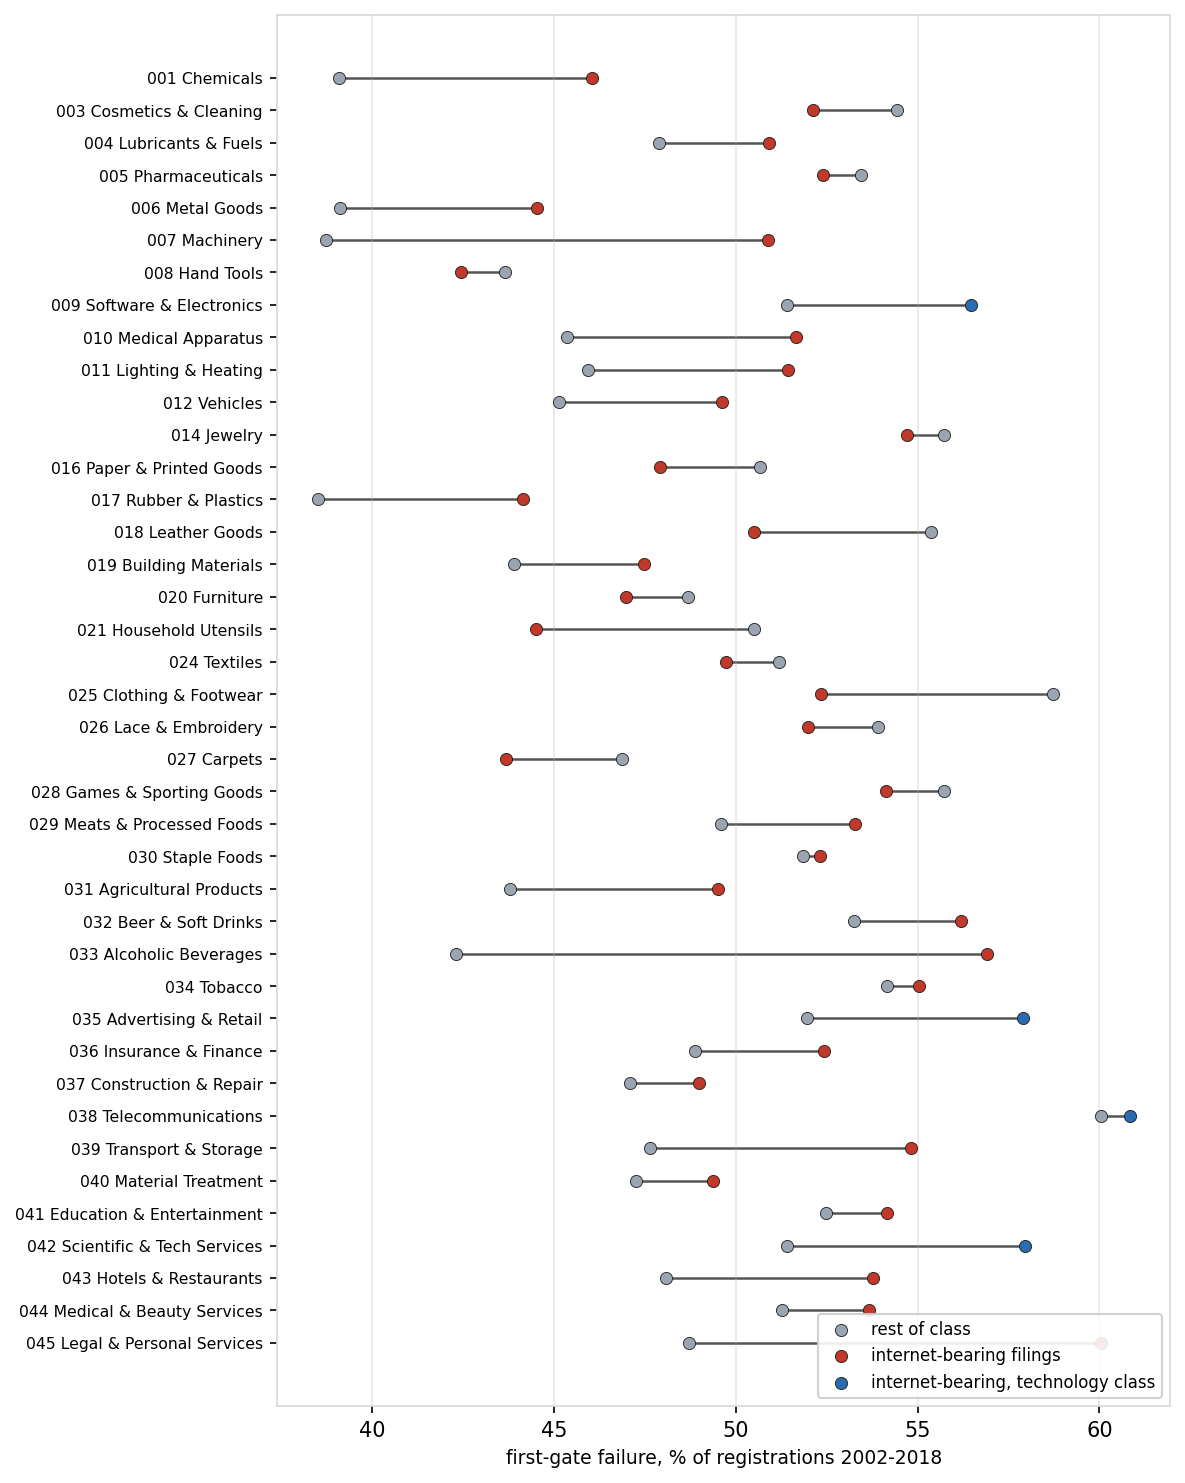
\includegraphics[width=0.8\textwidth]{results/internet_breakout.png}
\caption{First-gate failure of internet-bearing registrations (red; blue in
the four technology classes) against the rest of the same class (grey),
registrations 2002--2018.}
\label{fig:internet}
\end{figure}

Three patterns are in the table. In the industrial goods classes,
internet-bearing registrations fail the gate far more often than their
class: chemicals 46.1\% against 39.1\%, metal goods 44.5\% against 39.1\%,
machinery 50.9\% against 38.7\%, rubber and plastics 44.1\% against 38.5\%,
vehicles 49.6\% against 45.1\%, medical apparatus 51.7\% against 45.4\%. A
web-based business registering in an engineering class fails at the rate of
a software registration (51.4\%), not at the rate of its class. In the
consumer goods classes the sign reverses: internet-bearing registrations in
clothing fail 52.4\% against 58.7\% for the class, in carpets 43.7\% against
46.9\%, in household utensils 44.5\% against 50.5\%, in paper and printed
goods 47.9\% against 50.7\%. Online sellers of consumer goods outlast the
class's other registrants. In every service class the internet-bearing
filings fail more often, by one to eleven points, and most in legal and
personal services (60.1\% against 48.7\%) and advertising and retail
(57.9\% against 52.0\%). Pooled, internet-bearing registrations fail at
57.9\% against 51.8\% in the technology classes, 54.2\% against 49.9\% in
the other service classes, and 50.1\% against 50.1\% in goods classes, where
the industrial and consumer differences cancel.

Registration runs the other way in goods. Internet-bearing applications in
goods classes reach registration 59.5\% of the time against 56.0\% for the
rest, and in the technology and service classes slightly less often than the
rest. The examiner's step and the market's step do not agree about these
filings: an internet description in a goods class is a little more likely to
be granted and, in the industrial classes, a good deal more likely to be
cancelled for non-use six years later.

The classification system has faced this question and twice declined to
make the internet a class. Before 2002, internet and computer services
accumulated in class 42, whose heading then ended ``services that cannot be
classified in other classes''; the Nice Union's Committee of Experts
restructured it in the eighth edition, effective 1 January 2002, by
narrowing 42 to scientific and technological services and moving the rest
into three new classes (43--45), organised by the kind of service rather
than by the technology.\footnote{Nice Classification, 8th edition (WIPO,
2002); the USPTO's guidance describes the class-42 restructuring. The
eighth edition took effect in the middle of the era swing of
Section~\ref{sec:eras}.} The question returned with virtual goods: the
twelfth edition, effective 1 January 2023, classifies downloadable virtual
goods and NFT-authenticated files in class 9 and distributes
metaverse-related services across the existing service classes, again
declining a new class.\footnote{Nice Classification, 12th edition (WIPO,
2023).} The pattern in Table~\ref{tab:internet} bears on that choice.
Internet-bearing filings in a goods class survive or fail at rates closer
to the technology classes than to their own class, so for the outcome this
paper measures, the technology overlay carries more information than the
class assignment it is filed under. A classification built for scope of
protection has no reason to track survival; but a reader using Nice classes
as industry controls, as this paper and the literature do, should know that
the internet cuts across them.

\subsection{Why the rest of the paper conditions on reaching the first gate}\label{sec:filter}

Registration is not a neutral filter on language, so every estimate below
conditions on it. Completion is an inverse-U in atypicality: applicants whose
language sits far from their category in either direction follow through least
often, and the penalty is larger for the conventional tail than the unusual
one. Pooling granted and abandoned filings therefore mixes what examination
does to a description with what the market does to the product, and the
resulting gradients are attenuated and in places reversed
(Appendix~\ref{sec:robust_uncond}).

Conditioning would be the wrong move if abandonment were usually a pause
rather than an ending --- if firms reworked refused applications and refiled
them, the same commercial intent would be counted once as a failure and again
as a success. It is not. Among 2.28 million abandoned applications, only
3.6\% are followed within six years by the same owner filing the same mark
again in the same class, and only 1.5\% by one that then registers. Crediting
every successful refiling as an eventual registration moves the inverse-U in
atypicality from a depth of $+2.91$pp to $+2.85$pp. Abandonment is
overwhelmingly terminal, and what the registration step selects on is
therefore a property of the filing rather than an artifact of counting.

The refilings that do occur show what an applicant changes on a second
attempt, and that is a weakness of the construct. Among the 42{,}115
abandoned applications whose owner later registered the same mark in the
same class, 74\% carry a different goods/services description the second
time. Scoring each registration on the text it was first tried with and on
the text it registered with gives the direction of the change. Both
self-filers and represented owners rewrite toward the class's typical
description: originals in the most atypical fifth lose $0.39$ nats of
atypicality, and originals in the most conventional fifth gain $0.16$.
Refilings that reuse the identical text move by less than $0.01$ at every
position, so the convergence is in the writing, not in the reference
windows. Representation changes the extent but not the direction: owners
who hire counsel for the second attempt rewrite most often (82\%) and their
descriptions lengthen by 16\%; counsel rewriting their own earlier draft
rewrite least often (72\%) and shorten by 4\%
(Appendix~\ref{app:refile}). Lead barely moves once the windows' shift
with the later date is taken out: about $0.02$, a sixth of a standard
deviation.

Applicants therefore adjust their descriptions to resemble what the class
already files. A registered description is in part a conformed one, and the
atypicality of registered marks is compressed relative to the atypicality of
what applicants first wrote. Every estimate on registered marks is an
estimate on conformed language. For these 42{,}115 cases the first text is
observed; for an applicant who conformed before filing it is not, and the
compression cannot be bounded. The cases themselves move nothing: refiled
registrations are $1.1$\% of the gate sample, they fail it slightly less
often than other registrations (51.7\% against 52.8\%), and the
within-class-and-year contrast is $+2.25$pp with them and without them.
Which text predicts their gate cannot be told on 34{,}551 cases ($+0.9$pp
on the rewrite, $+0.7$pp on the original, both with standard errors near
$0.8$pp).

What examination rewards is a middling specificity --- concrete enough to
survive a definiteness objection, conventional enough to avoid a
likelihood-of-confusion refusal. Completion runs from 46.6\% at the least
atypical end to about 58\% in the middle and back to 53.4\% at the most
atypical; Appendix~\ref{app:registration} gives the profile on each axis and
why familiarity alone cannot produce it. The rest of this section is about what
happens to marks after the office has granted them.


Sections~\ref{sec:resolution} and~\ref{sec:secevents} are therefore
confined to registrations, and within them to the first use-proof gate and to
what follows it. A mark that never registered left the record by the
applicant's inaction in nine cases of ten, before any product met a
customer; a mark that registered and then failed the gate names a product
that was in commerce and is not. The second is the outcome the paper is
about. Appendix~\ref{sec:robust_uncond} shows what the pooled analysis looks like
without the condition: the registration step's shape is stamped onto every
later outcome, and the gradients the conditioned analysis finds are
attenuated and in places reversed.
